
\documentclass{beamer}
\usecolortheme{dove}
\setbeamertemplate{navigation symbols}{}
\usepackage{amsmath,amssymb,amsfonts,amsthm, multicol, subfigure, color}
\usepackage{bm}
\usepackage{graphicx}
\usepackage{tabularx}
\usepackage{booktabs}
\usepackage{hyperref}
\usepackage{pdfpages}
\usepackage{xcolor}
\definecolor{seagreen}{RGB}{46, 139, 87}
\definecolor{darkgold}{RGB}{255, 184, 28}
\definecolor{gold}{RGB}{255, 209, 0}
%\definecolor{blue}{RGB}{50, 131, 191}
% define blue as color 1
\definecolor{color1}{RGB}{0, 0, 255}
% define seagreen as color 2
\definecolor{color2}{RGB}{46, 139, 87}
\def\independenT#1#2{\mathrel{\rlap{$#1#2$}\mkern2mu{#1#2}}}
\newcommand\indep{\protect\mathpalette{\protect\independenT}{\perp}}
\def\log{\text{log}}
\newcommand\logit{\text{logit}}
\newcommand\iid{\stackrel{\text{iid}}{\sim}}
\newcommand\E{\text{E}}
\newcommand\V{\text{V}}
\renewcommand\P{\text{P}}
\newcommand{\Cov}{\text{Cov}}
\newcommand{\Cor}{\text{Cor}}
\newcommand\doop{\texttt{do}}
\usepackage{stackrel}
\usepackage{tikz}
\usetikzlibrary{arrows,shapes.arrows,positioning,shapes,patterns,calc}
\newcommand\slideref[1]{\vskip .1cm \tiny \textcolor{gray}{{#1}}}
\newcommand\red[1]{\color{red}#1}
\newcommand\blue[1]{\color{blue}#1}
\newcommand\gray[1]{\color{gray}#1}
\newcommand\seagreen[1]{\color{seagreen}#1}
\newcommand\purple[1]{\color{purple}#1}
\newcommand\orange[1]{\color{orange}#1}
\newcommand\black[1]{\color{black}#1}
\newcommand\white[1]{\color{white}#1}
\newcommand\teal[1]{\color{teal}#1}
\newcommand\magenta[1]{\color{magenta}#1}
\newcommand\Fuchsia[1]{\color{Fuchsia}#1}
\newcommand\BlueGreen[1]{\color{BlueGreen}#1}
\newcommand\bblue[1]{\textcolor{blue}{\textbf{#1}}}
\newcommand\bred[1]{\textcolor{red}{\textbf{#1}}}
\newcommand\bgray[1]{\textcolor{gray}{\textbf{#1}}}
\newcommand\bgreen[1]{\textcolor{seagreen}{\textbf{#1}}}
\newcommand\bref[2]{\href{#1}{\color{blue}{#2}}}
\colorlet{lightgray}{gray!40}
\pgfdeclarelayer{bg}    % declare background layer for tikz
\pgfsetlayers{bg,main} % order layers for tikz
%\newcommand\mycite[1]{\begin{scriptsize}\textcolor{darkgray}{(#1)}\end{scriptsize}}
\newcommand\mycite[1]{\begin{scriptsize}\begin{itemize}\item \textcolor{gray}{#1}\end{itemize}\end{scriptsize}}
\newcommand{\tcframe}{\frame{
%\small{
\only<1|handout:0>{\tableofcontents}
\only<2|handout:1>{\tableofcontents[currentsubsection]}}
%}
}

\usepackage[round]{natbib}
\bibliographystyle{humannat-mod}
\setbeamertemplate{enumerate items}[default]
\usepackage{mathtools}
\usepackage{ulem}

% Need to add examples

\newcommand{\goalsframe}{\begin{frame}{Learning goals for today}
At the end of class, you will be able to:
\begin{enumerate}
\item Define principal strata
\item Understand how they address a post-treatment problem
\item Make assumptions to draw inference about a latent stratum
\end{enumerate} \vskip .2in
\end{frame}}

\title{title}
\author{Lundberg \& Cho}
\date{21 Sep 2023\\Cornell Causal Reading Group}

\begin{document}

%\maketitle

\begin{frame}
\begin{tikzpicture}[x = \textwidth, y = \textheight]
\node at (0,0) {};
\node at (1,1) {};
\node[anchor = north west, align = left, font = \Huge] (t) at (0,.9) {\textbf{Non-existent}\\\textbf{outcomes}\\in research\\on inequality};
\node[anchor = north west, align = left, font = \huge] at (0, .4) {A causal approach};
\node[anchor = north east, gray, font = {\Large\bf}] (ian) at (1, .9) {Ian Lundberg};
\node[anchor = north east, gray, align = right] at (ian.south east) {Cornell Information Science\\ilundberg@cornell.edu};
\node[anchor = north east, gray, font = {\Large\bf}] (soonhong) at (1, .7) {Soonhong Cho};
\node[anchor = north east, gray, align = right] at (soonhong.south east) {UCLA Political Science\\soonhongcho@g.ucla.edu};
\node[anchor = north east, gray, align = right] at (1,.43) {Cornell Inequality\\Discussion Group\\16 Oct 2023};
\node[anchor = south east, align = right] (try) at (1,.05) {Try our (beta) R package!\\\bref{https://ilundberg.github.io/pstratreg/github_doc/_book/index.html}{ilundberg.github.io/pstratreg}};
\node[anchor = south west, align = left] at (0,.05) {Replication\\code \bref{https://github.com/ilundberg/replication/tree/master/pstratreg\_ex}{here}};
\draw[thick] (try.south west) -- (try.north west) -- (try.north east);
\end{tikzpicture}
\end{frame}

\begin{frame}
\bgray{Idea}\\
Outcomes that do not exist can hide inequality \vskip .2in
\bgray{Plan}
\begin{itemize}
\item one concrete setting
\item general methodological tools
\item open questions
\end{itemize}
\end{frame}

\begin{frame}
Parenthood reduces hourly wages for women \mycite{Budig \& England 2001; Gough \& Noonan 2013} \vskip .1in
and increases wages for men \mycite{Killewald 2013; Yu \& Hara 2021}
\vskip .2in \pause
The motherhood wage penalty may be disappearing over time \mycite{Pal \& Waldfogel 2016; Buchmann \& McDaniel 2016; but see Jee et al. 2019}
\end{frame}

% MAYA
\begin{frame}
\begin{tikzpicture}[x = \textwidth, y = \textheight]
\node at (0,0) {};
\node at (1,1) {};
\node[font = \huge] at (.5,.8) {Maya};
\pause
\node (a1) at (.35, .7) {if a mother};
\draw[thick] (a1.south west) -- (a1.south east);
\node (a0) at (.6, .7) {if not};
\draw[thick] (a0.south west) -- (a0.south east);
\node[font = \Large] at (.5,.7) {${}-{}$};
\node[font = \Large] at (.725,.7) {${}={}$};
\node (effect) at (.85,.7) {effect};
\draw[thick] (effect.south west) -- (effect.south east);
\pause
\node[anchor = east] (emp) at (.2, .6) {employment};
\node[anchor = east] (wage) at (.2, .5) {wage};
\node[font = \Large] at (.5,.6) {${}-{}$};
\node[font = \Large] at (.725,.6) {${}={}$};
\node[font = \Large] at (.5,.5) {${}-{}$};
\node[font = \Large] at (.725,.5) {${}={}$};
\pause
\node (bcase1) at (.35,.6) {\includegraphics[width = .3in]{bcase}}; 
\pause
%\draw[line cap = round, line width = 2pt, red] (bcase1.north west) -- (bcase1.south east);
%\draw[line cap = round, line width = 2pt, red] (bcase1.north east) -- (bcase1.south west);
\node (bcase2) at (.6,.6) {\includegraphics[width = .3in]{bcase}};
\pause
\node[font = \Large] at (.85, .6) {$0$};
\pause
% Wage effect
\node[font = \Large] at (.35, .5) {\$30};
\pause
\node[font = \Large] at (.6, .5) {\$40};
\pause
\node[font = \Large] at (.85, .5) {$-\$10$};
\end{tikzpicture}
\end{frame}

% MIA
\begin{frame}
\begin{tikzpicture}[x = \textwidth, y = \textheight]
\node at (0,0) {};
\node at (1,1) {};
\node[font = \huge] at (.5,.8) {Mia};
\node (a1) at (.35, .7) {if a mother};
\draw[thick] (a1.south west) -- (a1.south east);
\node (a0) at (.6, .7) {if not};
\draw[thick] (a0.south west) -- (a0.south east);
\node[font = \Large] at (.5,.7) {${}-{}$};
\node[font = \Large] at (.725,.7) {${}={}$};
\node (effect) at (.85,.7) {effect};
\draw[thick] (effect.south west) -- (effect.south east);
\node[anchor = east] (emp) at (.2, .6) {employment};
\node[anchor = east] (wage) at (.2, .5) {wage};
\node[font = \Large] at (.5,.6) {${}-{}$};
\node[font = \Large] at (.725,.6) {${}={}$};
\node[font = \Large] at (.5,.5) {${}-{}$};
\node[font = \Large] at (.725,.5) {${}={}$};
\pause
\node (bcase1) at (.35,.6) {\includegraphics[width = .3in]{bcase}}; 
\draw[line cap = round, line width = 2pt, red] (bcase1.north west) -- (bcase1.south east);
\draw[line cap = round, line width = 2pt, red] (bcase1.north east) -- (bcase1.south west);
\pause
\node (bcase2) at (.6,.6) {\includegraphics[width = .3in]{bcase}};
\pause
\node[font = \Large] at (.85, .6) {$-1$};
\pause
% Wage effect
\node[font = \Large] at (.35, .5) {??};
\pause
\node[font = \Large] at (.6, .5) {\$20};
\pause
\node[font = \Large] at (.85, .5) {??};
\pause
\node[anchor = south west, font = {\gray\footnotesize}, align = left] at (0,.1) {\textbf{Principal Stratification}\\\href{https://doi.org/10.1111/j.0006-341X.2002.00021.x}{Frangakis \& Rubin 2002}; \href{https://doi.org/10.3102/10769986028004353}{Zhang \& Rubin 2003}\\For an intro, see \href{https://doi.org/10.1080/19345747.2017.1379576}{Miratrix et al. 2018}};
\end{tikzpicture}
\end{frame}

% Four women
\begin{frame}
\begin{tikzpicture}[x = \textwidth, y = \textheight]
\node at (0,0) {};
\node at (1,1) {};
% MAYA
\node at (.25,.75) {\resizebox{.5\textwidth}{!}{
\begin{tikzpicture}[x = \textwidth, y = \textheight]
\node at (.25,.85) {};
\node at (1,.45) {};
\node<1-2>[font = \huge] at (.5,.8) {Maya};
\node<3->[font = \huge] at (.5,.8) {Maya is a Mother};
\node (a1) at (.35, .7) {if a mother};
\draw[thick] (a1.south west) -- (a1.south east);
\node (a0) at (.6, .7) {if not};
\draw[thick] (a0.south west) -- (a0.south east);
\node[font = \Large] at (.5,.7) {${}-{}$};
\node[font = \Large] at (.725,.7) {${}={}$};
\node (effect) at (.85,.7) {effect};
\draw[thick] (effect.south west) -- (effect.south east);
%\node[anchor = east] (emp) at (.2, .6) {employment};
%\node[anchor = east] (wage) at (.2, .5) {wage};
\node[font = \Large] at (.5,.6) {${}-{}$};
\node[font = \Large] at (.725,.6) {${}={}$};
\node[font = \Large] at (.5,.5) {${}-{}$};
\node[font = \Large] at (.725,.5) {${}={}$};
\node (bcase1) at (.35,.6) {\includegraphics[width = .3in]{bcase}}; 
%\draw[line cap = round, line width = 2pt, red] (bcase1.north west) -- (bcase1.south east);
%\draw[line cap = round, line width = 2pt, red] (bcase1.north east) -- (bcase1.south west);
\node (bcase2) at (.6,.6) {\includegraphics[width = .3in]{bcase}};
\node[font = \Large] at (.85, .6) {$0$};
% Wage effect
\node[font = \Large] at (.35, .5) {\$30};
\node[font = \Large] at (.6, .5) {\$40};
\node[font = \Large] at (.85, .5) {$-\$10$};
% GRAY OUT COUNTERFACTUAL
\draw<4->[fill = white, fill opacity = .85, draw = white] (.53,.45) rectangle (.7,.75);
\draw<4->[fill = white, fill opacity = .85, draw = white] (.75,.45) rectangle (.95,.75);
\end{tikzpicture}
}};
% MIA
\node at (.25, .45) {\resizebox{.5\textwidth}{!}{
\begin{tikzpicture}[x = \textwidth, y = \textheight]
\node at (.25,.85) {};
\node at (1,.45) {};
\node<1-2>[font = \huge] at (.5,.8) {Mia};
\node<3->[font = \huge] at (.5,.8) {Mia is a Mother};
\node (a1) at (.35, .7) {if a mother};
\draw[thick] (a1.south west) -- (a1.south east);
\node (a0) at (.6, .7) {if not};
\draw[thick] (a0.south west) -- (a0.south east);
\node[font = \Large] at (.5,.7) {${}-{}$};
\node[font = \Large] at (.725,.7) {${}={}$};
\node (effect) at (.85,.7) {effect};
\draw[thick] (effect.south west) -- (effect.south east);
%\node[anchor = east] (emp) at (.2, .6) {employment};
%\node[anchor = east] (wage) at (.2, .5) {wage};
\node[font = \Large] at (.5,.6) {${}-{}$};
\node[font = \Large] at (.725,.6) {${}={}$};
\node[font = \Large] at (.5,.5) {${}-{}$};
\node[font = \Large] at (.725,.5) {${}={}$};
\node (bcase1) at (.35,.6) {\includegraphics[width = .3in]{bcase}}; 
\draw[line cap = round, line width = 2pt, red] (bcase1.north west) -- (bcase1.south east);
\draw[line cap = round, line width = 2pt, red] (bcase1.north east) -- (bcase1.south west);
\node (bcase2) at (.6,.6) {\includegraphics[width = .3in]{bcase}};
\node[font = \Large] at (.85, .6) {$-1$};
% Wage effect
\node[font = \Large] at (.35, .5) {??};
\node[font = \Large] at (.6, .5) {\$20};
\node[font = \Large] at (.85, .5) {??};
% GRAY OUT COUNTERFACTUAL
\draw<4->[fill = white, fill opacity = .85, draw = white] (.53,.45) rectangle (.7,.75);
\draw<4->[fill = white, fill opacity = .85, draw = white] (.75,.45) rectangle (.95,.75);
\end{tikzpicture}
}};
\only<2->{
% NANCY
\node at (.75,.75) {\resizebox{.5\textwidth}{!}{
\begin{tikzpicture}[x = \textwidth, y = \textheight]
\node at (.25,.85) {};
\node at (1,.45) {};
\node<1-2>[font = \huge] at (.5,.8) {Nancy};
\node<3->[font = \huge] at (.56,.8) {Nancy is a Non-Mother};
\node (a1) at (.35, .7) {if a mother};
\draw[thick] (a1.south west) -- (a1.south east);
\node (a0) at (.6, .7) {if not};
\draw[thick] (a0.south west) -- (a0.south east);
\node[font = \Large] at (.5,.7) {${}-{}$};
\node[font = \Large] at (.725,.7) {${}={}$};
\node (effect) at (.85,.7) {effect};
\draw[thick] (effect.south west) -- (effect.south east);
%\node[anchor = east] (emp) at (.2, .6) {employment};
%\node[anchor = east] (wage) at (.2, .5) {wage};
\node[font = \Large] at (.5,.6) {${}-{}$};
\node[font = \Large] at (.725,.6) {${}={}$};
\node[font = \Large] at (.5,.5) {${}-{}$};
\node[font = \Large] at (.725,.5) {${}={}$};
\node (bcase1) at (.35,.6) {\includegraphics[width = .3in]{bcase}}; 
%\draw[line cap = round, line width = 2pt, red] (bcase1.north west) -- (bcase1.south east);
%\draw[line cap = round, line width = 2pt, red] (bcase1.north east) -- (bcase1.south west);
\node (bcase2) at (.6,.6) {\includegraphics[width = .3in]{bcase}};
\node[font = \Large] at (.85, .6) {$0$};
% Wage effect
\node[font = \Large] at (.35, .5) {\$30};
\node[font = \Large] at (.6, .5) {\$40};
\node[font = \Large] at (.85, .5) {$-\$10$};
% GRAY OUT COUNTERFACTUAL
\draw<4->[fill = white, fill opacity = .85, draw = white] (.25,.45) rectangle (.45,.75);
\draw<4->[fill = white, fill opacity = .85, draw = white] (.75,.45) rectangle (.95,.75);
\end{tikzpicture}
}};
% NIA
\node at (.75, .45) {\resizebox{.5\textwidth}{!}{
\begin{tikzpicture}[x = \textwidth, y = \textheight]
\node at (.25,.85) {};
\node at (1,.45) {};
\node<1-2>[font = \huge] at (.5,.8) {Nia};
\node<3->[font = \huge] at (.53,.8) {Nia is a Non-Mother};
\node (a1) at (.35, .7) {if a mother};
\draw[thick] (a1.south west) -- (a1.south east);
\node (a0) at (.6, .7) {if not};
\draw[thick] (a0.south west) -- (a0.south east);
\node[font = \Large] at (.5,.7) {${}-{}$};
\node[font = \Large] at (.725,.7) {${}={}$};
\node (effect) at (.85,.7) {effect};
\draw[thick] (effect.south west) -- (effect.south east);
%\node[anchor = east] (emp) at (.2, .6) {employment};
%\node[anchor = east] (wage) at (.2, .5) {wage};
\node[font = \Large] at (.5,.6) {${}-{}$};
\node[font = \Large] at (.725,.6) {${}={}$};
\node[font = \Large] at (.5,.5) {${}-{}$};
\node[font = \Large] at (.725,.5) {${}={}$};
\node (bcase1) at (.35,.6) {\includegraphics[width = .3in]{bcase}}; 
\draw[line cap = round, line width = 2pt, red] (bcase1.north west) -- (bcase1.south east);
\draw[line cap = round, line width = 2pt, red] (bcase1.north east) -- (bcase1.south west);
\node (bcase2) at (.6,.6) {\includegraphics[width = .3in]{bcase}};
\node[font = \Large] at (.85, .6) {$-1$};
% Wage effect
\node[font = \Large] at (.35, .5) {??};
\node[font = \Large] at (.6, .5) {\$20};
\node[font = \Large] at (.85, .5) {??};
% GRAY OUT COUNTERFACTUAL
\draw<4->[fill = white, fill opacity = .85, draw = white] (.25,.45) rectangle (.45,.75);
\draw<4->[fill = white, fill opacity = .85, draw = white] (.75,.45) rectangle (.95,.75);\end{tikzpicture}
}};
}
\node<5-8>[rotate = 35, gray, fill = white, draw = gray, rounded corners, line width = 1.5pt] at (.25,.45) {DROPPED};
\node<7-8>[rotate = 35, gray, fill = white, draw = gray, rounded corners, line width = 1.5pt, align = center] at (.75,.45) {SHOULD ALSO\\DROP};
\only<6>{
\node[font = \bf] at (.22,.25) {Average Observed};
\node[font = \bf] at (.72,.25) {Average Observed};
\node[font = \huge] at (.22,.15) {\$30};
\node[font = \huge] at (.72,.15) {\$30};
}
\draw<8->[fill = color1, draw = white, fill opacity = .2] (0,.6) rectangle (.95,.88);
\draw<8->[fill = color1, draw = white, fill opacity = .2] (0,.9) rectangle (.06,.96);
\node<8->[font = \bf, anchor = west] at (.07,.93) {subgroup: always employed};
\draw<9->[fill = color2, draw = white, fill opacity = .2] (0,.3) rectangle (.95,.6);
\draw<9->[fill = color2, draw = white, fill opacity = .2] (0,.22) rectangle (.06,.28);
\node<9->[font = \bf, anchor = west] at (.07,.25) {subgroup: motherhood blocks employment};
\end{tikzpicture}
\end{frame}

\begin{frame}
\begin{tikzpicture}[x = \textwidth, y = \textheight]
\node at (0,0) {};
\node at (1,1) {};
\node[anchor = north east] at (.18,.95) {\textbf{Goal}};
\node[anchor = north west] at (.18,.95) {Motherhood wage effect among the \blue{always-employed}};
\node[anchor = north, align = center, font = \footnotesize, blue] at (.85,.85) {women who\\would be employed if a mom\\and\\would be employed if not};
\draw[->, thick, blue] (.85, .85) -- (.85, .88);
\draw[thick, blue] (.75, .89) -- (.95,.89);
\pause
\node[anchor = north east] at (.18,.88) {\textbf{Difficulty}};
\node[anchor = north west] at (.18,.88) {Who are those people?};
\pause
\node at (.2,.75) {Mother?};
\node at (.34,.75) {Wage};
\node[anchor = east] at (.12,.69) {Maya};
\node at (.2,.69) {Yes};
\node at (.34,.69) {\$30};
\node[anchor = east] at (.12,.63) {Mia};
\node at (.2,.63) {Yes};
\node at (.34,.63) {??};
\node[anchor = east] at (.12,.57) {Nancy};
\node at (.2,.57) {No};
\node at (.34,.57) {\$40};
\node[anchor = east] at (.12,.51) {Nia};
\node at (.2,.51) {No};
\node at (.34,.51) {\$20};
\pause
\draw[thick] (0,.63) -- (.4,.63);
\pause
\node[anchor = north west, align = left] at (0,.45) {\textbf{Assumption.}\\Employed mothers would still be\\employed even if they had no children};
\pause
\draw[fill = color1, fill opacity = .2, draw = white] (0,.66) rectangle (.4,.72);
\pause
\foreach \i in {0,.1,.2,.3} {
\draw<7>[fill = color1, fill opacity = .2, draw opacity = 0] (\i,.48) rectangle (\i + .05,.6);
\draw<7>[fill = color2, fill opacity = .2, draw opacity = 0] (\i + .05,.48) rectangle (\i + .1,.6);
}
%\draw[->, thick] (.45,.54) -- (.4,.56);
%\draw[->, thick] (.45,.54) -- (.4,.52);
%\pause
%\node[anchor = west] at (.45,.54) {One is always employed};
\pause
\node[anchor = north west, align = left] at (0,.25) {\textbf{Bound.}\\Report the highest and lowest estimates\\consistent with the data};
\draw[thick] (.66,.1) -- (.66,.47) -- (1,.47);
\node[anchor = north west, align = left] at (.67, .45) {Estimated Effect\\of Motherhood};
\node[anchor = north west] at (.67, .3) {Upper Bound:};
\node[anchor = north west] at (.67, .22) {Lower Bound:};
\draw<9>[fill = color1, fill opacity = .2, draw = white] (0,.48) rectangle (.4,.54);
\node<9->[anchor = north west] at (.9,.3) {$+\$10$};
\draw<10>[fill = color1, fill opacity = .2, draw = white] (0,.54) rectangle (.4,.6);
\node<10->[anchor = north west] at (.9,.22) {$-\$10$};
% below just keeps a click where the shading is gone
\node<11> at (0,0) {};
\end{tikzpicture}
\end{frame}

\begin{frame}

In practice,
\begin{itemize}
\item motherhood is not randomized
\item identical people do not exist
\end{itemize} \vskip .3in
Our contribution: Model-based estimates
\end{frame}

\begin{frame}{Data: NLSY97}
\resizebox{\textwidth}{!}{\begin{tikzpicture}[x = \textwidth, y = .9\textheight]
\node at (0,0) {};
\node at (1,1) {};
\node at (-.18,.5) {};
\node[anchor = east, font = {\Large\bf}] (parents) at (.3,.8) {Parents};
\node[anchor = north east, black, font = \footnotesize, align = left] at (parents.south east) {2,181 mothers\\2,055 fathers};
\node[black, font = {\Large\bf}] at (.4,.9) {Pre};
\node[black, font = {\Large\bf}] (birth) at (.6,.9) {Birth};
\node[black, font = {\Large\bf}, anchor = south] at (birth.north) {First};
\node[black, font = {\Large\bf}] at (.8,.9) {Post};
\node[black, font = \Huge] (ppre) at (.4,.8) {$\bullet$};
\node[black, font = \Huge] (pbirth) at (.6,.8) {$\bullet$};
\node[black, font = \Huge] (ppost) at (.8,.8) {$\bullet$};
\draw[->, line width = 2pt, black] (ppre) to node[midway, below, align = center] {9+\\months} (pbirth);
\draw[->, line width = 2pt, black] (pbirth) to node[midway, below, align = center] {12+\\months} (ppost);
\pause
\node[anchor = east, font = {\Large\bf}] (nonparents) at (.3,.6) {Non-Parents};
\node[anchor = north east, black, font = \footnotesize, align = left] at (nonparents.south east) {\begin{tabular}{rrr}
& person-periods & persons \\
women & 20,578 & 2,796 \\
men & 25,921 &  3,439
\end{tabular}};
\node[black, font = \Huge] (npre) at (.4,.6) {$\bullet$};
\node[black, font = \Huge] (npost) at (.8,.6) {$\bullet$};
\node[black, font = \footnotesize, anchor = north west, align = center] at (npost.north east) {allowed to\\subsequently\\have a\\child};
\draw[->, line width = 2pt, black] (npre) to node[midway, below, align = center] {21+\\months} (npost);
\pause
\node[black, anchor = north, align = center] at (.4,.35) {measure\\confounders};
\node[black, anchor = north, align = center] at (.8,.35) {measure\\outcome};
\draw[->, thick, black] (.4,.35) -- (.4,.45);
\draw[->, thick, black] (.8,.35) -- (.8,.45);
\end{tikzpicture}}

\end{frame}

\begin{frame}{Causal assumptions}
\begin{center}
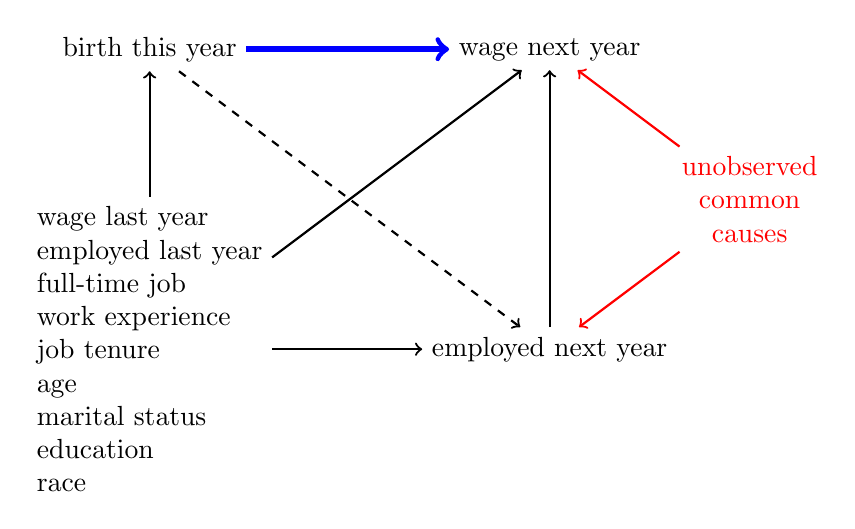
\begin{tikzpicture}[x = 2in, y = 1.5in]
\node (a) at (0,0) {birth this year};
\node (y) at (1,0) {wage next year};
\draw[->, line width = 2pt, blue] (a) -- (y);
\pause
\node (m) at (1,-1) {employed next year};
\draw[->, thick, dashed] (a) -- (m);
\draw[->, thick] (m) -- (y);
\pause
\node[red, align = center] (u) at (1.5,-.5) {unobserved\\common\\causes};
\draw[->, thick, red] (u) -- (m);
\draw[->, thick, red] (u) -- (y);
\pause
\node[align = left] (x) at (0,-1) {wage last year\\employed last year\\full-time job\\work experience\\job tenure\\age\\marital status\\education\\race};
\draw[->, thick] (x) -- (a);
\draw[->, thick] (x) -- (m);
\draw[->, thick] (x) -- (y);
\end{tikzpicture}
\end{center}
\end{frame}

\begin{frame}{Modeling strategy}

\begin{enumerate}
\item Logit of employment given motherhood and confounders
\begin{itemize}
\item Estimate the proportion always-employed at each $\vec{X},A$
\end{itemize}
\item OLS model of wage given motherhood and confounders
\begin{itemize}
\item Predict wage under motherhood \hfill (no modifications)
\item Predict wage under no motherhood \hfill (with bounding)
\end{itemize}
\end{enumerate}

\end{frame}

\begin{frame}{Modeling strategy}

\begin{tikzpicture}
\node<1> at (0,0) {\includegraphics[width = .8\textwidth]{../figures/teach_nonmother}};
\node<2> at (0,0) {\includegraphics[width = .8\textwidth]{../figures/teach_nonmother_upper_0}};
\node<3> at (0,0) {\includegraphics[width = .8\textwidth]{../figures/teach_nonmother_upper_1}};
\node<4> at (0,0) {\includegraphics[width = .8\textwidth]{../figures/teach_nonmother_lower_0}};
\node<5> at (0,0) {\includegraphics[width = .8\textwidth]{../figures/teach_nonmother_lower_1}};
\end{tikzpicture}

\end{frame}

\begin{frame}{Results}

\begin{tikzpicture}[x = \textwidth,y = .9\textheight]
\node at (0,0) {};
\node at (1,1) {};
\node<1>[anchor = west] at (0,.7) {\includegraphics[width = \textwidth]{../figures/parenthood_employment_1}};
\node<2>[anchor = west] at (0,.7) {\includegraphics[width = \textwidth]{../figures/parenthood_employment_2}};
\node<3>[anchor = west] at (0,.7) {\includegraphics[width = \textwidth]{../figures/parenthood_employment_3}};
\node<4>[anchor = west] at (0,.7) {\includegraphics[width = \textwidth]{../figures/parenthood_employment_conditional_1}};
\node<5>[anchor = west] at (0,.7) {\includegraphics[width = \textwidth]{../figures/parenthood_employment_conditional_2}};
\node<6>[anchor = west] at (0,.7) {\includegraphics[width = \textwidth]{../figures/parenthood_employment_conditional}};
\end{tikzpicture}

\end{frame}

\begin{frame}{Results}
\begin{tikzpicture}[x = \textwidth, y = .9\textheight]
\node at (0,0) {};
\node at (1,1) {};
\node<1>[anchor = west] at (0,.7) {\includegraphics[width = .9\textwidth]{../figures/motherhood_1}};
\node<2>[anchor = west] at (0,.7) {\includegraphics[width = .9\textwidth]{../figures/motherhood_2}};
\node<3>[anchor = west] at (0,.7) {\includegraphics[width = .9\textwidth]{../figures/motherhood_4}};
\node<4>[anchor = west] at (0,.7) {\includegraphics[width = .9\textwidth]{../figures/motherhood_5}};
\node<5>[anchor = west] at (0,.7) {\includegraphics[width = .9\textwidth]{../figures/motherhood_6}};
\node<4->[anchor = west] at (0,.3) {If you believe the};
\draw<4->[fill = color1] (.31,.28) rectangle (.35,.33);
\node<4->[anchor = west, align = left] at (.35, .3) {\textbf{lowest}-earning};;
\node<5->[anchor = west, align = left] at (.6, .3) {or};;
\draw<5->[fill = color2] (.66,.28) rectangle (.7,.33);
\node<5->[anchor = west, align = left] at (.7, .3) {\textbf{highest}-earning};
\node<4->[anchor = north west, align = left] at (0, .25) {non-mothers would stop paid employment if they had a child};
%\node<5->[anchor = west, align = left, font = \footnotesize] at (.1, .25) {if you believe the\\\textbf{lowest}-earning non-mothers\\would stop working if\\they became mothers};
%\node<5->[anchor = west, align = left, font = \footnotesize] at (.1, .25) {if the \textbf{lowest}-earning\\non-moms would stop working\\if counterfactually moms};
%\node<6->[anchor = west, align = left, font = \footnotesize] at (.6, .25) {if you believe the\\\textbf{highest}-earning non-mothers\\would stop working if\\they became mothers};
\end{tikzpicture}
\end{frame}



\begin{frame}{What we know that we did not know before}

\pause
%Has the motherhood wage penalty disappeared?
%\mycite{Pal \& Waldfogel 2016; Buchmann \& McDaniel 2016} \vskip .2in
\bgray{We knew}\\
in recent years, motherhood only weakly predicts pay\textsuperscript{*}\vskip .2in
\pause
\begin{center}
\textsuperscript{*}among the employed
\end{center} \vskip .2in \pause
This fact is consistent with two stories \vskip .05in \pause
\begin{enumerate}
\item motherhood's causal effect on pay is small \pause \vskip .05in
\begin{center}
\textbf{or}
\end{center} \vskip .05in
\item employed non-mothers the wrong comparison population \pause
\begin{itemize}
\item lowest-earning non-mothers might stop paid work with a child
\end{itemize}
\end{enumerate}

\end{frame}

\begin{frame}{What we know that we did not know before}
\begin{tikzpicture}[x = \textwidth, y = .9\textheight]
\node at (0,0) {};
\node at (1,1) {};
\node[anchor = north west, align = left] at (0,.95) {
We know how to think\\about outcomes that\\\textbf{don't exist}};
\onslide<2->{
\node[outer sep = 0pt] (bcase1) at (.1,.65) {\includegraphics[width = .3in]{bcase}};
\draw[line cap = round, line width = 2pt, red] (bcase1.north west) -- (bcase1.south east);
\draw[line cap = round, line width = 2pt, red] (bcase1.north east) -- (bcase1.south west);
\node at (.17,.65) {$-$};
\node at (.24,.65) {\includegraphics[width = .3in]{bcase}};
\node at (.3,.65) {$=$};
\node at (.35,.65) {$-1$};
\node at (.1,.55) {??};
\node at (.17,.55) {$-$};
\node at (.24,.55) {$\$25$};
\node at (.3,.55) {$=$};
\node at (.35,.55) {??};
}
\node<3->[anchor = north west] at (.5,.95) {in the labor market};
\node<3->[anchor = north west, font = \small] at (.52,.9) {--- some people are not employed};
\node<4->[anchor = north west] at (.5,.83) {in intergenerational mobility};
\node<4->[anchor = north west, font = \small] at (.52,.78) {--- some people have no kids};
\node<5->[anchor = north west] at (.5,.7) {in assortative mating};
\node<5->[anchor = north west, font = \small] at (.52,.65) {--- some people have no spouse};
\node<6->[anchor = south west] at (0,.1) {\includegraphics[width = .45\textwidth]{../figures/pstratreg_site}};
\node<7->[anchor = south west] at (.5,0) {\includegraphics[height = .5\textheight]{../figures/pstratreg_help}};
\end{tikzpicture}
\end{frame}



\begin{frame}

\huge{Appendix}

\end{frame}

\begin{frame}{Sample restrictions: Persons}

\resizebox{\textwidth}{!}{
\begin{tabular}{rllll}
& Mothers & Non-Mothers & Fathers & Non-Fathers \\
\hline
All & 2,999 & 3,746 & 2,662 & 4,200 \\
18+ at pre-period & 2,315 & 2,832 & 2,273 & 3,522 \\
Observed in windows\textsuperscript{*} & 2,098 & 2,830 & 2,029 & 3,517 \\
Non-missing wage if employed & 1,985 & 2,794 & 1,837 & 3,436 \\
\hline
\end{tabular}
} \vskip .2in

\scalebox{.7}{
\begin{minipage}{\textwidth}
\textsuperscript{*} Requirement is
\begin{itemize}
\item parents: observed at
\begin{itemize}
\item pre-birth: 3 years to 9 months before
\item post-birth: 1--3 years after
\end{itemize}
\item for non-parents, two observations
\begin{itemize}
\item at least 1 year + 9 months apart
\item no more than 6 years apart
\end{itemize}
\end{itemize}
\end{minipage}
}
\end{frame}

\begin{frame}{Sample restrictions: Person-Periods}

\resizebox{\textwidth}{!}{
\begin{tabular}{rllll}
& Mothers & Non-Mothers & Fathers & Non-Fathers \\
\hline
All & 2,999 & 31,510 & 2,662 & 39,325 \\
18+ at pre-period & 2,315 & 21,743 & 2,273 & 28,159 \\
Observed in windows\textsuperscript{*} & 2,098 & 21,704 & 2,029 & 29,135 \\
Non-missing wage if employed & 1,985 & 20,543 & 1,837 & 25,902 \\
\hline
\end{tabular}
} \vskip .2in

\scalebox{.7}{
\begin{minipage}{\textwidth}
\textsuperscript{*} Requirement is
\begin{itemize}
\item parents: observed at
\begin{itemize}
\item pre-birth: 3 years to 9 months before
\item post-birth: 1--3 years after
\end{itemize}
\item for non-parents, two observations
\begin{itemize}
\item at least 1 year + 9 months apart
\item no more than 6 years apart
\end{itemize}
\end{itemize}
\end{minipage}
}
\end{frame}

\begin{frame}{Variable definitions}
\begin{itemize}
\item $A$ treatment: first birth occurs
\item $Y$ outcome: log hourly wage in 2022 dollars
\begin{itemize}
\item including tips, overtime bonuses
\item includes non-hourly workers
\item for the job current at interview date
\end{itemize}
\item $\vec{X}$ confounders
\begin{itemize}
\item log(wage in pre-period)
\item employed in pre-period
\item full time (35+ hours) in pre-period current job
\item log(years of full-time work experience + 1), from weekly arrays
\item log(years of tenure in current job + 1), from job roster
\item age + age squared
\item marital status (married with spouse present, cohabiting, other)
\item education (less than high school, high school degree, 2-year college degree, 4-year college degree)
\item race (Hispanic, non-Hispanic Black, other)
\end{itemize}
\end{itemize}
\end{frame}

\begin{frame}{Statistical models: Mediator (employment)}

$A$ indicates parenthood\\
$M = 1$ indicates employment\\
$\vec{X}$ are confounders
$$\begin{aligned}
\text{logit}\left(P(M =1 \mid \vec{X},A)\right) &= \alpha + \vec{X}'\vec\gamma + A\left(\beta + \vec{X}'\vec\eta\right)
\end{aligned}$$ \vskip .05in
\bgray{Conditional average effect on mediator (employment)}
$$\begin{aligned}
\hat{P}(M^1 =1 \mid \vec{X},A) &= \text{logit}^{-1}\left(\hat\alpha + \vec{X}'\hat{\vec\gamma} + 1\times \left(\hat\beta + \vec{X}'\hat{\vec\eta}\right)\right) \\
\hat{P}(M^0 =1 \mid \vec{X},A) &= \text{logit}^{-1}\left(\hat\alpha + \vec{X}'\hat{\vec\gamma} + 0\times \left(\hat\beta + \vec{X}'\hat{\vec\eta}\right)\right)
\end{aligned}$$
Conditional Average Effect = Top $-$ Bottom

\end{frame}

\begin{frame}{Statistical models: Outcome (wage)}

$A$ indicates parenthood. $M = 1$ indicates employment.\\
$Y$ is log hourly wage. $\vec{X}$ are confounders.
$$\begin{aligned}
Y \mid \vec{X},A,M=1 &\sim \text{Normal}\left(\mu(\vec{X},A),\sigma^2(\vec{X},A)\right)\\
\mu\left(\vec{X},A\right) &= \lambda + \vec{X}'{\vec\nu} + A\left(\tau  +\vec{X}'{\vec\delta}\right) \\
\log\left[\sigma^2\left(\vec{X},A\right)\right] &= \xi + \vec{X}'{\vec\psi} + A\omega
\end{aligned}$$ \vskip .05in
Estimate by
\begin{itemize}
\item for $\mu(\vec{X},A)$, estimate by OLS with $Y$ as the outcome
\item then we calculate the residual $\hat\epsilon = Y - \hat{Y}$
\item for $\sigma^2(\vec{X},A)$, estimate by Gamma GLM with a log link with $\hat\epsilon^2$ as the outcome \hfill \textcolor{gray}{(Western \& Bloome 2009)}
\end{itemize}

\end{frame}

\begin{frame}{Statistical models: Effects on wage}

\begin{enumerate}
\item At the $\vec{X}$ of each unit, simulate
\begin{itemize}
\item $Y^1 \sim \text{Normal}\left(\mu(\vec{X},A = 1),\sigma^2(\vec{X},A = 1)\right)$
\item $Y^0 \sim \text{Normal}\left(\mu(\vec{X},A = 0),\sigma^2(\vec{X},A = 0)\right)$
\end{itemize}
\item Remove the upper (lower) portion at this $\vec{X}$ value estimated to be the not-always-employed
\item Estimate the mean of the simulated values
\item Repeat for every unit
\end{enumerate}
\end{frame}

\begin{frame}{Normality of residuals}

\includegraphics[width = .48\textwidth]{../figures/motherhood_resid_hist}
\includegraphics[width = .48\textwidth]{../figures/motherhood_qq}

\end{frame}

\begin{frame}{Histogram: Wage}

\includegraphics[width = .48\textwidth]{../figures/motherhood_wage}
\includegraphics[width = .48\textwidth]{../figures/motherhood_log_wage}

\end{frame}

\begin{frame}{Alternative: Utility functions}

Alternative solution: Code the unemployed people with a wage
\begin{itemize}
\item if unemployed, then code with minimum wage
\end{itemize} \vskip .1in
This works if you believe a utility function
$$
U = \begin{cases}
\text{log}\left(\text{min wage}\right) &\text{if not employed} \\
\text{log}\left(\text{wage}\right) &\text{if employed}
\end{cases}
$$
But if it is just a convenience
\begin{itemize}
\item then it does not bound effects on $Y$
\item you might miss the real story
\begin{itemize}
\item if half the sample was not employed, would you do this?
\end{itemize}
\end{itemize}

\end{frame}

\begin{frame}[t]{Alternative: Heckman selection}
\vskip .1in
\bgray{Premise:} Everyone has a wage offer. Non-employed don't take it. \vskip .05in
\bgray{Goal:} Infer about everyone, despite sample selection. \vskip .15in
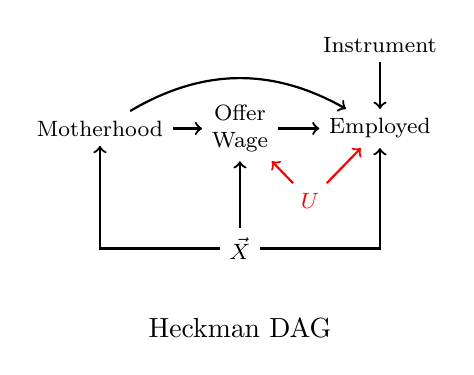
\begin{tikzpicture}[x = .7in, y = .6in]
\node[anchor = north] (title) at (0,-1.5) {Heckman DAG};
\node[font = \footnotesize] (a) at (-1,0) {Motherhood};
\node[font = \footnotesize, align = center] (y) at (0,0) {Offer\\Wage};
\node[font = \footnotesize] (s) at (1,0) {Employed};
\node[font = \footnotesize] (x) at (0,-1) {$\vec{X}$};
\node[font = \footnotesize] (z) at (1,.7) {Instrument};
\draw[->, thick] (a) -- (y);
\draw[->, thick] (a) to[bend left] (s);
\draw[->, thick] (y) -- (s);
\draw[->, thick] (x) -- (-1,-1) -- (a);
\draw[->, thick] (x) -- (1,-1) -- (s);
\draw[->, thick] (x) -- (y);
\draw[->, thick] (z) -- (s);
\node[font = \footnotesize, red] (u) at (.5,-.6) {$U$};
\draw[->, thick, red] (u) -- (y);
\draw[->, thick, red] (u) -- (s);
\end{tikzpicture}
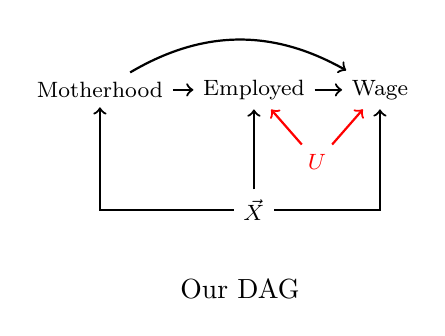
\begin{tikzpicture}[x = .7in, y = .6in]
\node[anchor = north] (title) at (0,-1.5) {Our DAG};
\node[font = \footnotesize] (a) at (-1,0) {Motherhood};
\node[font = \footnotesize] (m) at (.1,0) {Employed};
\node[font = \footnotesize] (y) at (1,0) {Wage};
\node[font = \footnotesize] (x) at (.1,-1) {$\vec{X}$};
\draw[->, thick] (x) -- (-1,-1) -- (a);
\draw[->, thick] (x) -- (1,-1) -- (y);
\draw[->, thick] (x) -- (m);
\draw[->, thick] (a) -- (m);
\draw[->, thick] (a) to[bend left] (y);
\draw[->, thick] (m) -- (y);
\node[font = \footnotesize, red] (u) at (.55,-.6) {$U$};
\draw[->, thick, red] (u) -- (y);
\draw[->, thick, red] (u) -- (m);
\end{tikzpicture}

\end{frame}

\begin{frame}{Fatherhood effects}
\includegraphics[width = .8\textwidth]{../figures/fatherhood}
\end{frame}

\begin{frame}{Histogram: Age at birth}

\includegraphics[width = .7\textwidth]{../figures/motherhood_age_at_birth}

\end{frame}

\begin{frame}{Histogram: Observation timing around birth}

\includegraphics[width = .7\textwidth]{../figures/motherhood_age_gaps}

\end{frame}

\begin{frame}{Histogram: Age of wage measurement}

\includegraphics[width = .7\textwidth]{../figures/motherhood_age_wage}

\end{frame}

\begin{frame}{Histogram: Year of wage measurement}

\includegraphics[width = .7\textwidth]{../figures/motherhood_year_wage}

\end{frame}

\end{document}